\documentclass[11pt,a4paper]{article}

% ------------------------------------------------------------------ packages
\usepackage[margin=2.3cm]{geometry}
\usepackage[T1]{fontenc}
\usepackage{lmodern}
\usepackage{microtype}
\usepackage{amsmath,amssymb}
\usepackage{booktabs}
\usepackage{float}
\usepackage{tabularx}
\usepackage{enumitem}
\usepackage{xcolor}
\usepackage{caption}
\usepackage{tikz}
\usetikzlibrary{positioning,arrows.meta,shapes.geometric,fit,calc,backgrounds,decorations.pathreplacing}
\usepackage{pgfplots}
\pgfplotsset{compat=1.17}
\usepackage[colorlinks=true,linkcolor=blue!50!black,urlcolor=blue!50!black]{hyperref}

\definecolor{accent}{RGB}{31,95,170}
\definecolor{good}{RGB}{46,125,50}
\definecolor{bad}{RGB}{183,28,28}
\definecolor{soft}{RGB}{240,244,250}

\setlist{itemsep=2pt,topsep=4pt}
\setlength{\parskip}{4pt}
\setlength{\parindent}{0pt}

\newcommand{\code}[1]{\texttt{#1}}
\newcommand{\step}[2]{\paragraph{Step #1 -- #2.}}

\tikzset{
  box/.style={draw, rounded corners=3pt, align=center, minimum height=9mm,
              inner sep=4pt, font=\small},
  hot/.style={box, draw=accent, fill=accent!10, line width=0.9pt},
  arr/.style={-{Stealth[length=2.2mm]}, thick},
  lab/.style={font=\scriptsize, align=center, text=black!70},
}

% ------------------------------------------------------------------ title
\title{\textbf{RiskGate-ML}\\[4pt]
  \large A pre-trade risk gateway with on-chip machine learning\\
  How the hardware and the software work, step by step}
\author{Your Name}
\date{20 November 2026}

\begin{document}
\maketitle

\begin{abstract}
\noindent
RiskGate-ML is a silicon chip, designed for the Tiny Tapeout programme, that sits between
a bank's trading algorithms and the stock exchange and decides, for every order, whether it
may go out. It combines five hard risk rules that regulators require with a small
machine-learning model that catches suspicious orders the rules miss. Each decision takes
one clock cycle, 40 nanoseconds. On held-out test data, the rules alone block 43.8\% of
the orders from injected incidents (runaway algorithms, fat-finger errors, price
manipulation, quote stuffing). With the on-chip model, the chip blocks 87.6\%, while the model
wrongly blocks only 0.8\% of legitimate orders. The model is the provably best possible
tree that fits in the chip, found by mixed-integer optimisation. This report explains,
in plain terms, what the software does on a laptop and what the hardware does on the chip.
\end{abstract}

\tableofcontents
\newpage

% ==================================================================
\section{The problem}

Most stock trading today is done by computer programs, called \emph{algorithms}, that can send
thousands of orders a second. When one of them breaks, it can lose a fortune before a person
notices. In 2012, Knight Capital lost about \$440 million in 45 minutes because a faulty
program kept sending orders and nothing stopped it.

Regulators therefore require a \textbf{pre-trade risk check}: a gatekeeper that inspects every
order before it leaves the bank and blocks the dangerous ones. In Canada this is National
Instrument 23-103; in the United States, SEC Rule 15c3-5. Two things make it hard:

\begin{itemize}
  \item \textbf{Speed.} The check delays every single order, and in trading microseconds matter.
        Software checks take microseconds and their timing varies. A dedicated chip decides in a
        fixed, tiny time.
  \item \textbf{Fixed rules miss things.} A rule such as ``no order above 200 shares'' only
        catches dangers someone thought of in advance. An order that is a little too big,
        a little off-price and a little too fast passes every rule, although the combination
        is suspicious.
\end{itemize}

RiskGate-ML addresses both. The hard rules run in hardware, and a small machine-learning
model runs right beside them to catch suspicious combinations. The model can only
\emph{add} rejections: it can never approve an order that broke a rule.

% ==================================================================
\section{The big picture}

The project has two halves that meet in one small file (Figure~\ref{fig:big}).

\begin{itemize}
  \item \textbf{Software}, in Python on a laptop, creates realistic trading data, learns from it,
        and finds the best decision tree that fits in the chip. This happens once, before the chip
        is used, and again whenever the model is retrained.
  \item \textbf{Hardware}, in Verilog and manufactured as a chip, applies the rules and the
        tree to every order, live, in one clock cycle.
  \item \textbf{The bridge} is the trained tree: 7 yes/no questions and 8 answers. A small
        microcontroller on the Tiny Tapeout demo board loads it into the chip's registers at
        start-up. Because it lives in registers, not in the wiring, it can be retrained after the
        chip is made.
\end{itemize}

\begin{figure}[h]
\centering
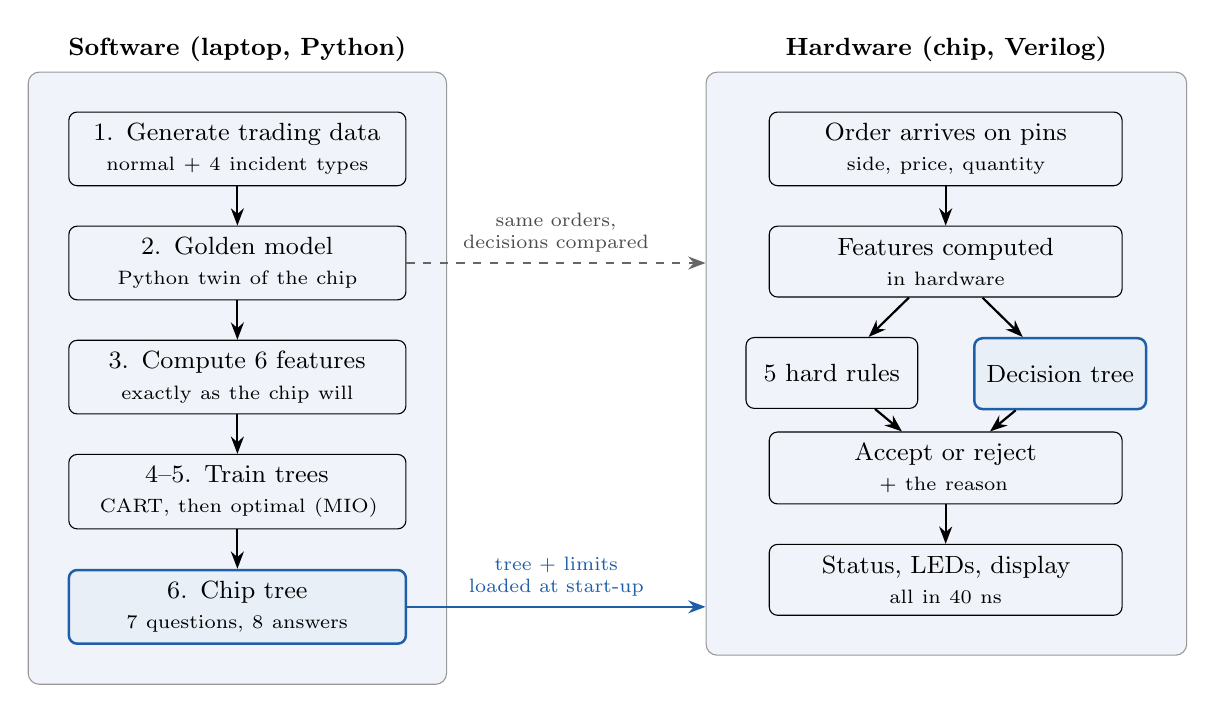
\begin{tikzpicture}[node distance=5mm and 8mm]
  % software column
  \node[box, text width=40mm] (gen) {1. Generate trading data\\\scriptsize normal + 4 incident types};
  \node[box, text width=40mm, below=of gen] (twin) {2. Golden model\\\scriptsize Python twin of the chip};
  \node[box, text width=40mm, below=of twin] (feat) {3. Compute 6 features\\\scriptsize exactly as the chip will};
  \node[box, text width=40mm, below=of feat] (train) {4--5. Train trees\\\scriptsize CART, then optimal (MIO)};
  \node[hot, text width=40mm, below=of train] (tree) {6. Chip tree\\\scriptsize 7 questions, 8 answers};
  \draw[arr] (gen) -- (twin);
  \draw[arr] (twin) -- (feat);
  \draw[arr] (feat) -- (train);
  \draw[arr] (train) -- (tree);
  \begin{scope}[on background layer]
    \node[draw=black!40, rounded corners, fill=soft, fit=(gen)(tree), inner sep=5mm,
          label={[font=\small\bfseries]above:Software (laptop, Python)}] (sw) {};
  \end{scope}

  % hardware column
  \node[box, text width=42mm, right=46mm of gen] (pins) {Order arrives on pins\\\scriptsize side, price, quantity};
  \node[box, text width=42mm, below=of pins] (hf) {Features computed\\\scriptsize in hardware};
  \node[box, text width=19mm, below left=5mm and -19mm of hf] (rules) {5 hard rules};
  \node[hot, text width=19mm, below right=5mm and -19mm of hf] (htree) {Decision tree};
  \node[box, text width=42mm, below=17mm of hf] (dec) {Accept or reject\\\scriptsize + the reason};
  \node[box, text width=42mm, below=of dec] (out) {Status, LEDs, display\\\scriptsize all in 40 ns};
  \draw[arr] (pins) -- (hf);
  \draw[arr] (hf) -- (rules);
  \draw[arr] (hf) -- (htree);
  \draw[arr] (rules) -- (dec);
  \draw[arr] (htree) -- (dec);
  \draw[arr] (dec) -- (out);
  \begin{scope}[on background layer]
    \node[draw=black!40, rounded corners, fill=soft, fit=(pins)(rules)(htree)(out), inner sep=5mm,
          label={[font=\small\bfseries]above:Hardware (chip, Verilog)}] (hw) {};
  \end{scope}

  \draw[arr, accent] (tree.east) -- node[lab, above, text=accent] {tree + limits\\loaded at start-up}
        (tree.east -| hw.west);
  \draw[arr, dashed, black!60] (twin.east) -- node[lab, above] {same orders,\\decisions compared}
        (twin.east -| hw.west);
\end{tikzpicture}
\caption{What runs where. The software produces the tree once; the hardware uses it on every order.
The dashed link is the verification: the Python twin and the chip must agree on every decision.}
\label{fig:big}
\end{figure}

% ==================================================================
\section{The software, step by step}

All software is in the \code{ml/} folder. One command, \code{python train.py}, runs steps 3--8.

\step{1}{Create realistic trading data} (\code{generate\_data.py})
Real bank order data is private, so the program simulates it. It produces 60 \emph{sessions}.
Each is one trading algorithm's stream of about 330 orders over 3{,}000 time ticks
(roughly 3 seconds). Most orders come from a normal, well-behaved algorithm: prices near the
market price, sensible sizes, buying and selling in balance, sometimes in short legitimate bursts.
Into each session, 2--4 \emph{incidents} are injected, and every order in an incident is
labelled ``anomalous'' (Table~\ref{tab:scen}). In total there are 20{,}073 orders, 15\%
of them anomalous.

\begin{table}[H]
\centering\small
\begin{tabularx}{\linewidth}{@{}lXX@{}}
\toprule
Incident & What happens & Why rules struggle \\
\midrule
Runaway algorithm & Stuck in a loop, fires small same-side orders every 1--2 ticks (Knight Capital) & Each order is small and well priced \\
Fat-finger & One or two oversized orders, still under the size cap & Just inside every limit \\
Momentum ignition & A sequence on one side, walking the price away from the market & Each step is inside the price band \\
Quote stuffing & A flood of tiny orders alternating buy and sell & Tiny orders, no position builds up \\
\bottomrule
\end{tabularx}
\caption{The four injected incident types.}
\label{tab:scen}
\end{table}

\step{2}{Build a Python twin of the chip} (\code{riskgate\_model.py})
This ``golden model'' is a short Python program that behaves \emph{exactly} like the chip, bit for
bit: the same counters, the same rounding, the same limits. It serves two purposes: training
uses it to see the data the way the chip will, and testing uses it as the answer key the chip is
checked against.

\step{3}{Turn each order into six numbers (features)}
A model cannot look at an order directly. It looks at a few numbers that describe the order
and its context. The chip computes these itself, so they must be cheap to calculate in hardware:

\begin{table}[H]
\centering\small
\begin{tabularx}{\linewidth}{@{}clX@{}}
\toprule
& Feature & Plain meaning \\
\midrule
f0 & \code{price\_dev}   & How far the price is from the market reference price \\
f1 & \code{qty}          & Order size \\
f2 & \code{pos\_after}   & How big the bank's net position would be after this order (divided by 8) \\
f3 & \code{win\_count}   & Orders sent in the current rate window \\
f4 & \code{idle\_ticks}  & Time since the previous order \\
f5 & \code{side\_streak} & Orders in a row on the same side (buy, buy, buy, \ldots) \\
\bottomrule
\end{tabularx}
\caption{The six features. All are whole numbers from 0 to 255 (8 bits).}
\end{table}

The sixth feature was added after an experiment showed that a runaway algorithm's giveaway is
repetition on one side, which none of the first five captured. Adding it raised runaway detection
from 50\% to 81\% at the cost of 9 extra memory cells on the chip.

\step{4}{Train a baseline decision tree (CART)}
A \emph{decision tree} is a short chain of yes/no questions such as ``is the order size above 5?''
that ends in an answer: normal or anomalous. Trees suit hardware well, because each question is
a single comparison of two numbers. The chip has room for a tree three questions deep (7 questions,
8 answers). The standard method, CART in scikit-learn, builds the tree \emph{greedily}: it picks the
best first question, then the best second question under it, and so on, never reconsidering earlier
choices. Its settings are tuned on separate validation sessions. The baseline blocks 85.9\% of
anomalous orders on test data.

\step{5}{Find the provably best tree (mixed-integer optimisation)}
Greedy choices are usually good but not best, and CART optimises a statistical stand-in
(``purity'') rather than what the bank cares about. So the problem is stated exactly, as a
\emph{mixed-integer optimisation} (MIO): an optimisation problem with yes/no decision variables.

\begin{itemize}
  \item Decision variables: for each of the 7 question slots, which feature and threshold to use
        ($z_{n,s}\in\{0,1\}$), and for each of the 8 answers, normal or anomalous ($c_\ell\in\{0,1\}$).
  \item Objective: catch as many anomalous orders as possible \emph{that the hard rules let through}.
  \item Constraint: legitimate orders blocked by the model alone must stay at or below a budget
        $B$, set to 0.6\% of legitimate orders, a safety margin under the 1\% limit.
\end{itemize}

Written out, with $a_p$ and $n_p$ the anomalous and legitimate orders in group $p$, and
$w_{p\ell}$ meaning ``group $p$ lands in answer $\ell$'':
\begin{align*}
\max\;& \textstyle\sum_{p}\sum_{\ell} a_p\, y_{p\ell} \\
\text{s.t.}\;& \textstyle\sum_s z_{n,s} = 1 \ \ \forall n, \qquad \sum_\ell w_{p\ell} = 1 \ \ \forall p,\\
& w_{p\ell} \le \textstyle\sum_{s \text{ sends } p \text{ toward } \ell} z_{n,s} \quad \text{for each question } n \text{ on the path to } \ell,\\
& y_{p\ell} \le w_{p\ell},\quad y_{p\ell} \le c_\ell,\quad f_{p\ell} \ge w_{p\ell} + c_\ell - 1,\\
& \textstyle\sum_{p,\ell} n_p\, f_{p\ell} \le B .
\end{align*}

At the full data size this program has 115{,}000 variables, too many for the free solver available.
So the same problem is solved exactly by \emph{decomposition}. Each wrongly blocked order is given
a price $\lambda$. The budget then moves into the objective, the 8 answers no longer interact, and
every candidate tree can be scored at once with matrix multiplications. Trying a range of prices
gives two things:
\begin{itemize}
  \item the best tree that stays inside the budget, and
  \item a \textbf{proven upper bound}: no depth-3 tree can catch more than
        \[ \min_\lambda \Big[\max_{\text{tree}} \sum_\ell \max(0,\, A_\ell - \lambda N_\ell) + \lambda B\Big]. \]
\end{itemize}
The two methods were checked against each other on small problems the MIO solver can finish. On the
real data the optimal tree catches 1{,}055 anomalous orders against CART's 1{,}021, \emph{and}
wrongly blocks fewer legitimate ones (0.59\% against 0.79\%). It is proven to be within half an
order of the best possible tree. Figure~\ref{fig:tree} shows the tree the chip uses.

\begin{figure}[h]
\centering
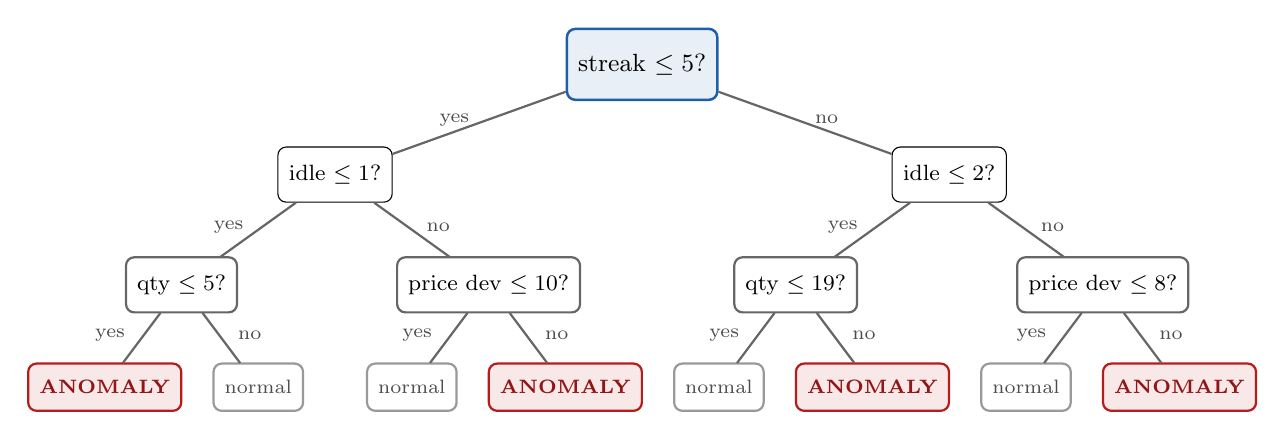
\begin{tikzpicture}[
  q/.style={box, minimum height=7mm, font=\footnotesize},
  an/.style={box, minimum height=6mm, font=\scriptsize\bfseries, draw=bad, fill=bad!10, text=bad!80!black},
  nl/.style={box, minimum height=6mm, font=\scriptsize, draw=black!40, text=black!70},
  level 1/.style={sibling distance=78mm, level distance=14mm},
  level 2/.style={sibling distance=39mm, level distance=14mm},
  level 3/.style={sibling distance=19.5mm, level distance=13mm},
  edge from parent/.style={draw, thick, black!60},
  yes/.style={lab, left=3pt, pos=0.45},
  no/.style={lab, right=3pt, pos=0.45}
]
\node[q, hot] {streak $\le 5$?}
  child { node[q] {idle $\le 1$?}
    child { node[q] {qty $\le 5$?}
      child { node[an] {ANOMALY} edge from parent node[yes] {yes} }
      child { node[nl] {normal} edge from parent node[no] {no} }
      edge from parent node[yes] {yes} }
    child { node[q] {price dev $\le 10$?}
      child { node[nl] {normal} edge from parent node[yes] {yes} }
      child { node[an] {ANOMALY} edge from parent node[no] {no} }
      edge from parent node[no] {no} }
    edge from parent node[yes] {yes} }
  child { node[q] {idle $\le 2$?}
    child { node[q] {qty $\le 19$?}
      child { node[nl] {normal} edge from parent node[yes] {yes} }
      child { node[an] {ANOMALY} edge from parent node[no] {no} }
      edge from parent node[yes] {yes} }
    child { node[q] {price dev $\le 8$?}
      child { node[nl] {normal} edge from parent node[yes] {yes} }
      child { node[an] {ANOMALY} edge from parent node[no] {no} }
      edge from parent node[no] {no} }
    edge from parent node[no] {no} };
\end{tikzpicture}
\caption{The chip's tree. Left to right, the four anomaly answers catch: quote stuffing (tiny
orders, back-to-back); a far-off price (fat-finger or momentum); a runaway algorithm (a long
same-side streak, fast, real size); and momentum ignition (a long same-side streak walking the price).}
\label{fig:tree}
\end{figure}

\step{6}{Convert the tree to the chip's format}
The chip stores each question as a feature number (3 bits) and a threshold (8 bits), and the
answers as an 8-bit mask, 85 bits in all. The features are whole numbers, so a learned rule like
``qty $\le 19.5$'' becomes ``qty $\le 19$'' with no loss. The chip's tree therefore gives
\emph{exactly} the same answers as the trained one. (For the CART baseline this was checked on all
20{,}073 orders.)

\step{7}{Measure honestly}
The 60 sessions are split by session: 36 for training, 12 for validation and 12 for the final test,
so the test data is never seen during training. Testing replays each test session through the
golden model from start to finish. This matters because a blocked order does not change the bank's
position, so blocking changes the features of the orders after it. The test therefore measures the
whole system as it would run, not each order in isolation.

\step{8}{Export}
Training writes \code{tree.json} (the limits and the tree), a copy for the demo board, the metrics,
and one held-out session (307 orders) that the chip tests replay.

% ==================================================================
\section{The hardware, step by step}

The chip (\code{src/project.v}, \code{src/rg\_tree.v}) runs on a 25\,MHz clock, one tick every
40 nanoseconds. Its ``memory'' consists of 239 \emph{flip-flops}, each holding one bit, and its
``thinking'' consists of about 1{,}600 logic gates wired between them. Figure~\ref{fig:datapath}
shows the path an order takes.

\begin{figure}[h]
\centering
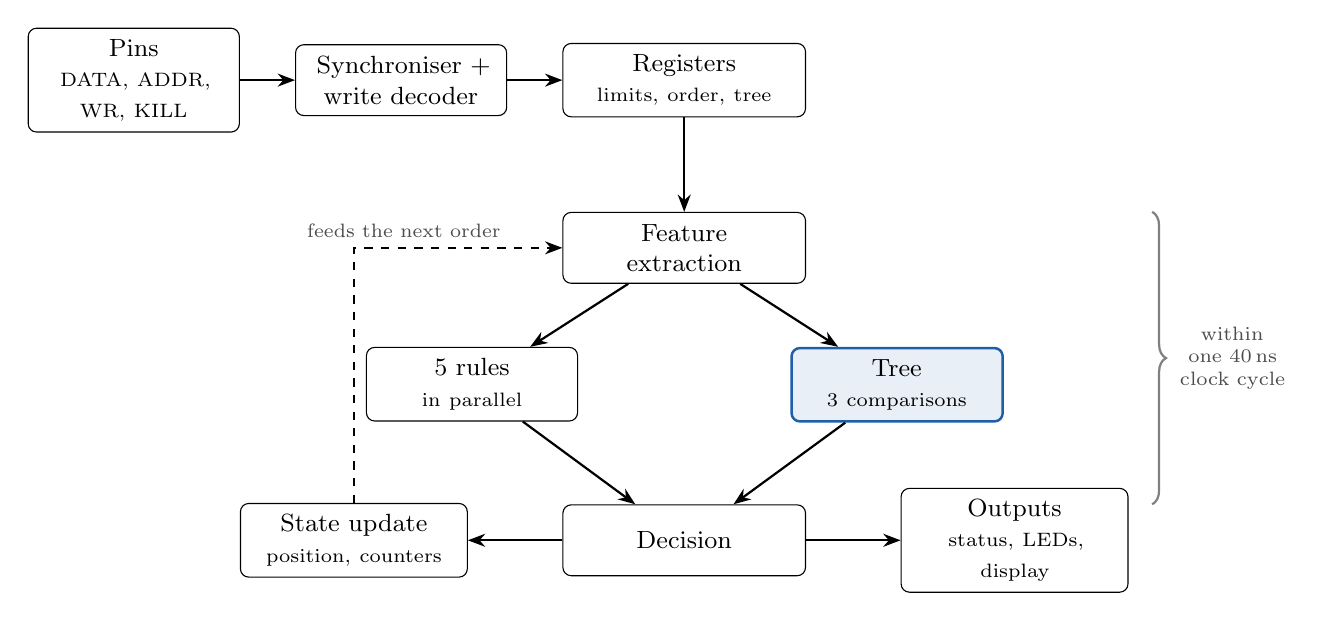
\begin{tikzpicture}[node distance=6mm and 7mm]
  \node[box, text width=24mm] (pins) {Pins\\\scriptsize DATA, ADDR, WR, KILL};
  \node[box, text width=24mm, right=of pins] (sync) {Synchroniser +\\write decoder};
  \node[box, text width=28mm, right=of sync] (regs) {Registers\\\scriptsize limits, order, tree};
  \node[box, text width=28mm, below=12mm of regs] (feat) {Feature\\extraction};
  \node[box, text width=24mm, below left=8mm and -2mm of feat] (rules) {5 rules\\\scriptsize in parallel};
  \node[hot, text width=24mm, below right=8mm and -2mm of feat] (tree) {Tree\\\scriptsize 3 comparisons};
  \node[box, text width=28mm, below=28mm of feat] (dec) {Decision};
  \node[box, text width=26mm, left=12mm of dec] (state) {State update\\\scriptsize position, counters};
  \node[box, text width=26mm, right=12mm of dec] (out) {Outputs\\\scriptsize status, LEDs, display};
  \draw[arr] (pins) -- (sync);
  \draw[arr] (sync) -- (regs);
  \draw[arr] (regs) -- (feat);
  \draw[arr] (feat) -- (rules);
  \draw[arr] (feat) -- (tree);
  \draw[arr] (rules) -- (dec);
  \draw[arr] (tree) -- (dec);
  \draw[arr] (dec) -- (state);
  \draw[arr] (dec) -- (out);
  \draw[arr, dashed] (state.north) |- node[lab, above, pos=0.62] {feeds the next order} (feat.west);
  \draw[decorate, decoration={brace, amplitude=5pt}, thick, black!50]
        ($(out.east |- feat.north)+(3mm,0)$) -- ($(out.east |- dec.north)+(3mm,0)$)
        node[midway, right=4pt, lab, text width=15mm] {within one 40\,ns clock cycle};
\end{tikzpicture}
\caption{The chip's datapath. Everything from feature extraction to the decision is plain wiring
that settles within one clock cycle; the results are stored at the end of that cycle.}
\label{fig:datapath}
\end{figure}

\step{0}{Start-up: load the limits and the tree}
The demo board's microcontroller writes the limits (reference price, price band, maximum size,
position limit, rate limit and window) and the 7 questions and 8 answers into the chip's registers,
one byte at a time. This takes a few hundred writes, once.

\step{1}{Receive a byte safely}
To write a byte, the microcontroller puts an address (which register, 4 bits) and a value (8 bits)
on the pins, then raises the \code{WR} line. The microcontroller and the chip are not
synchronised, so \code{WR} may change at an awkward moment. The chip passes it through two
flip-flops in a row (a \emph{synchroniser}), which removes the risk of reading a half-changed
signal. A third flip-flop spots the moment \code{WR} goes from low to high. On that clock cycle,
the addressed register stores the byte.

\step{2}{Stage the order}
An order is three writes: \code{PRICE}, then \code{QTY}, then \code{SUBMIT} with the side
(buy or sell). The \code{SUBMIT} write triggers the decision.

\step{3}{Compute the six features (pure wiring)}
These circuits run continuously; their outputs are simply valid once the inputs are:
\begin{itemize}
  \item \textbf{price deviation}: a subtractor computes price $-$ reference, and its sign selects
        either it or its negative (an absolute value);
  \item \textbf{position after}: an adder or subtractor applies the order to the stored 12-bit
        position; the result is made positive, divided by 8 by dropping 3 bits, and capped at 255;
  \item \textbf{window count, idle time, streak}: these are counters that already hold the answer;
        the streak circuit also checks whether this order is on the same side as the last one.
\end{itemize}

\step{4}{Run the five hard rules, all at once}
Each rule is one comparator, a circuit that answers ``is A bigger than B?'':
kill switch on? price deviation $>$ band? size $= 0$ or $>$ limit? position after $>$ limit?
window count $\ge$ rate limit? The five work in parallel, side by side.

\step{5}{Ask the tree, one path only}
A tree has 7 questions, but any one order only meets 3 of them, one per level. So the chip needs
just 3 comparators instead of 7. The first compares the feature chosen by the root question with
its threshold. Its yes/no answer drives a \emph{multiplexer} (a digital switch) that selects which
second-level question to ask, and the second answer selects the third. The three answers together
form a 3-bit number, the leaf (answer) index, which looks up normal or anomalous in the 8-bit
answer mask.

\step{6}{Decide}
\[
\text{reject} \;=\; \text{any rule failed} \;\;\textbf{or}\;\; (\text{tree says anomalous} \textbf{ and } \text{ML enforcement on}).
\]
In \emph{shadow mode} (enforcement off), the model's opinion is recorded but nothing is blocked.
This is how a bank tests a new model before trusting it.

\step{7}{Update the state at the clock edge}
At the end of the cycle, flip-flops capture the results:
\begin{itemize}
  \item a status byte records which rules failed, whether the model flagged the order, and the verdict;
  \item the leaf number is kept, so every decision can be explained;
  \item the position is updated only if the order was accepted;
  \item the idle timer restarts, and the window counter and the streak counter step up.
\end{itemize}
These updated values feed into the features of the next order.

\step{8}{Report}
The microcontroller reads the status byte. Two pins drive ``accept'' and ``reject'' LEDs, and in
display mode the 7-segment display shows a letter: \textbf{A} accepted, \textbf{H} kill switch,
\textbf{P} price, \textbf{5} size, \textbf{L} position limit, \textbf{r} rate, \textbf{d} the
model; its dot lights when the model flagged the order.

\paragraph{Keeping time.}
A prescaler counter turns clock cycles into ticks, one every $2^n$ cycles ($n$ is programmable).
In \emph{manual time} mode, ticks happen only when the microcontroller asks for one. A recorded
trading session can then be replayed exactly, however slowly the microcontroller works. The tests
and the demo use this mode.

% ==================================================================
\section{How we know it works}

\begin{itemize}
  \item \textbf{13 automated tests} (cocotb, simulating the actual chip design) cover each rule,
        the kill switch pin, the tree in shadow and enforcing modes, every feature including
        saturation at 255, the display and LEDs, and the real-time clock.
  \item \textbf{Full-session replay.} A held-out session of 307 orders over 3{,}001 ticks is
        replayed into the simulated chip and into the Python twin. Every one of the 307 decisions,
        and the leaf behind each one, matches exactly.
  \item \textbf{Planted bugs.} To check that the tests can actually catch mistakes, seven
        deliberate bugs were planted one at a time (an off-by-one comparison, a wrong streak
        condition, a missing cap, and so on). The tests caught six. The seventh is a timing
        coincidence that only occurs in real-time mode, and it is listed as a known gap.
  \item \textbf{Only the pins.} The tests touch only the chip's pins, so the same tests can run
        unchanged on the final manufactured netlist in Tiny Tapeout's build.
\end{itemize}

% ==================================================================
\section{Results}

All figures are on the 12 held-out test sessions (38 incidents), replayed end to end.

\begin{table}[h]
\centering\small
\begin{tabularx}{\linewidth}{@{}Xrrr@{}}
\toprule
& Rules only & Rules + CART & \textbf{Rules + optimal tree} \\
\midrule
Anomalous orders blocked & 43.8\% & 85.9\% & \textbf{87.6\%} \\
Bad orders that got through before the first block, per incident & 7.5 & 2.4 & \textbf{2.2} \\
Legitimate orders blocked by the model alone & -- & 0.8\% & 0.8\% \\
\bottomrule
\end{tabularx}
\caption{Overall results. The budget for wrongly blocked legitimate orders is 1\%.}
\end{table}

\begin{figure}[h]
\centering
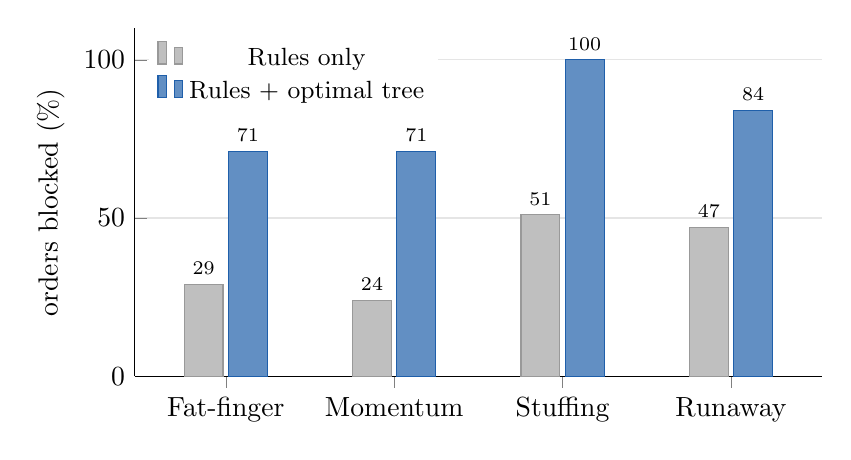
\begin{tikzpicture}
\begin{axis}[
  ybar, bar width=14pt, width=0.85\linewidth, height=6cm,
  ymin=0, ymax=110, ylabel={orders blocked (\%)},
  symbolic x coords={Fat-finger,Momentum,Stuffing,Runaway},
  xtick=data, enlarge x limits=0.18,
  nodes near coords, nodes near coords style={font=\scriptsize},
  legend style={at={(0.02,0.98)}, anchor=north west, font=\small, draw=none},
  axis lines*=left, ymajorgrids, grid style={black!10},
]
\addplot[fill=black!25, draw=black!40] coordinates
  {(Fat-finger,29) (Momentum,24) (Stuffing,51) (Runaway,47)};
\addplot[fill=accent!70, draw=accent] coordinates
  {(Fat-finger,71) (Momentum,71) (Stuffing,100) (Runaway,84)};
\legend{Rules only, Rules + optimal tree}
\end{axis}
\end{tikzpicture}
\caption{Blocked orders by incident type. The model helps most where incidents are built to stay
under every individual limit.}
\end{figure}

\paragraph{What limits accuracy.}
Experiments on the same data show where the ceiling is:
\begin{itemize}
  \item a deeper tree (4 levels) did \emph{not} help, and would double the tree's storage;
  \item adding the same-side streak feature helped a lot (72\% $\to$ 86\%);
  \item the optimal depth-3 tree is about 88\%, the most any tree of this size can reach here;
  \item a large boosted model with hundreds of trees reaches 94\%, but cannot fit in the chip.
\end{itemize}
The remaining gap is partly the chip's size limit and partly the labels themselves: every order
in an incident is marked anomalous, but the first few look exactly like normal trading.

% ==================================================================
\section{Limits and next steps}

\begin{itemize}
  \item \textbf{Synthetic data.} The trading data is simulated. The natural next step is to retrain
        on real order-book data. The chip itself would not change.
  \item \textbf{Not yet verified:} the exact chip area (expected to fit one Tiny Tapeout tile,
        but close to the limit), the tests on the final manufactured netlist, and the demo on a
        real board. Tiny Tapeout's GitHub build reports the first two.
  \item \textbf{Known test gap:} a window reset landing on the same clock cycle as an order, in
        real-time mode only.
  \item \textbf{Solver note:} the decomposition method can miss the true optimum by a few orders
        at some budgets. On the real data its certified gap was half an order.
\end{itemize}

% ==================================================================
\section{Glossary}

\begin{description}[style=nextline, leftmargin=0pt, labelsep=0pt]
  \item[Clock cycle] One beat of the chip's internal clock; here 40 nanoseconds (25 million per second).
  \item[Flip-flop] A circuit that stores one bit and updates it only at a clock beat.
  \item[Comparator] A circuit that tells whether one number is bigger than another.
  \item[Multiplexer] A digital switch that picks one of several inputs.
  \item[Register] A group of flip-flops holding a number, such as the position limit.
  \item[Synchroniser] Two flip-flops in a row that safely bring an outside signal into the chip's clock.
  \item[Feature] A number describing an order or its context, which the model looks at.
  \item[Decision tree] A chain of yes/no questions on features that ends in an answer.
  \item[CART] The standard greedy method for building decision trees (scikit-learn).
  \item[MIO] Mixed-integer optimisation: finding the best choice when some decisions are yes/no.
  \item[Lagrangian relaxation] Turning a hard limit into a price, so a hard problem splits into easy parts.
  \item[Golden model] A software twin of the chip, used as the answer key in testing.
  \item[Shadow mode] The model reports what it would block, but blocks nothing.
  \item[Tiny Tapeout] A programme that manufactures many small student and hobby chip designs together.
\end{description}

\end{document}
